\documentclass{beamer}
\usepackage[utf8]{inputenc}
\usepackage{graphicx, epsfig}
\usepackage{amsmath,mathrsfs,amsfonts,amssymb}
\usepackage{floatflt}
\usepackage{epic,ecltree}
\usepackage{mathtext}
\usepackage{fancybox}
\usepackage{fancyhdr}
\usepackage{multirow}
\usepackage{enumerate}
\usepackage{epstopdf}
\usepackage{multicol}
\usepackage{algorithm}
\usepackage[noend]{algorithmic}
\usepackage{tikz}
\usepackage{blindtext}
\usepackage{multido}
\usetheme{default}%{Singapore}%{Warsaw}%{Warsaw}%{Darmstadt}
\usecolortheme{default}

\setbeamerfont{title}{size=\Huge}
\setbeamertemplate{footline}[frame number]{}

\setbeamertemplate{section in toc}[sections numbered]

\makeatletter
\newcommand\HUGE{\@setfontsize\Huge{35}{40}}
\makeatother    

\setbeamerfont{title}{size=\HUGE}
\beamertemplatenavigationsymbolsempty

\usetikzlibrary{arrows,shapes,positioning,shadows,trees}

\newcommand\myfootnote[1]{%
  \vspace{-0.5cm}%
  \tikz[remember picture,overlay]
  \draw (current page.south west) +(1in + \oddsidemargin,0.5em)
  node[anchor=south west,inner sep=0pt]{\parbox{\textwidth}{%
      \rlap{\rule{10em}{0.4pt}}\raggedright\scriptsize \textit{#1}}};}

\newcommand\myfootnotewithlink[2]{%
  \vspace{-0.5cm}%
  \tikz[remember picture,overlay]
  \draw (current page.south west) +(1in + \oddsidemargin,0.5em)
  node[anchor=south west,inner sep=0pt]{\parbox{\textwidth}{%
      \rlap{\rule{10em}{0.4pt}}\raggedright\scriptsize\href{#1}{\textit{#2}}}};}

\AtBeginSection[]
      {
      	\begin{frame}{Outline}
      		\tableofcontents[currentsection]
      	\end{frame}
      }
      \AtBeginSubsection[]{
      	\begin{frame}{Outline}
      		\tableofcontents[currentsection,currentsubsection]
      	\end{frame}
}

\newcounter{noscounter} % Используется для nextonslide команды (обнуляется только на новом слайде)
\newcounter{pcounter} % Используется для pause команды (обнуляется после использования eqpause)
\newcounter{diffcounter} % Считает количество pause после формулы

\newcommand{\nextonslide}[1]{%
  \stepcounter{noscounter}% Прибавляем счетчик nextonslide
  \stepcounter{pcounter}% Прибавляем счетчик pause
  \stepcounter{diffcounter}% Прибавляем счетчик diffcounter
  \onslide<\value{noscounter}->{#1}% Отображаем аргумент в скобках на слайде с номером noscounter
}
\newcommand{\resetonslide}{%
    \setcounter{noscounter}{1}% Сбрасываем счетчик nextonslide
    \setcounter{pcounter}{1}% Сбрасываем счетчик pause
    \setcounter{diffcounter}{0}% Сбрасываем счетчик diffcounter
}

\newcommand{\eqpause}{%
  \multido{\i=1+1}{\value{pcounter}}{\pause}% Повторяем pcounter раз команду pause
  \stepcounter{noscounter}% Прибавляем счетчик nextonslide
  \setcounter{pcounter}{1}% Сбрасываем счетчик pause
}

\newcommand{\eqpausediff}{% Вспомогательная команда, запускается автоматически после формул
  \multido{\i=1+1}{\value{diffcounter}}{\pause}% Повторяем diffcounter раз команду pause
  \addtocounter{pcounter}{-\value{diffcounter}}% Вычитаем из pcounter количество сделанных pause
  \setcounter{diffcounter}{0}% Сбрасываем счетчик diffcounter
}

\newcommand\AtEndBoth[2]{% Применяем команду к multline и multline*
  \AtEndEnvironment{#1}{#2}%
  \AtEndEnvironment{#1*}{#2}%
}

\AtEndBoth{align}{\eqpausediff}
\AtEndBoth{equation}{\eqpausediff}
\AtEndBoth{multline}{\eqpausediff}

\addtobeamertemplate{frametitle}{\resetonslide}{}% На каждом слайде сбрасываем счетчики

% latin bold lower
\newcommand{\ba}{\mathbf{a}} 
\newcommand{\bc}{\mathbf{c}} 
\newcommand{\be}{\mathbf{e}} 
\newcommand{\bff}{\mathbf{f}} % \bf - for bold type
\newcommand{\bg}{\mathbf{g}} 
\newcommand{\bh}{\mathbf{h}} 
\newcommand{\bp}{\mathbf{p}} 
\newcommand{\bq}{\mathbf{q}} 
\newcommand{\bt}{\mathbf{t}} 
\newcommand{\bs}{\mathbf{s}} 
\newcommand{\bu}{\mathbf{u}} 
\newcommand{\bv}{\mathbf{v}} 
\newcommand{\bw}{\mathbf{w}} 
\newcommand{\bx}{\mathbf{x}} 
\newcommand{\by}{\mathbf{y}} 
\newcommand{\bz}{\mathbf{z}} 

% latin bold upper
\newcommand{\bA}{\mathbf{A}} 
\newcommand{\bB}{\mathbf{B}} 
\newcommand{\bC}{\mathbf{C}} 
\newcommand{\bG}{\mathbf{G}} 
\newcommand{\bI}{\mathbf{I}} 
\newcommand{\bJ}{\mathbf{J}} 
\newcommand{\bL}{\mathbf{L}} 
\newcommand{\bM}{\mathbf{M}} 
\newcommand{\bP}{\mathbf{P}}
\newcommand{\bQ}{\mathbf{Q}} 
\newcommand{\bR}{\mathbf{R}} 
\newcommand{\bT}{\mathbf{T}} 
\newcommand{\bU}{\mathbf{U}} 
\newcommand{\bV}{\mathbf{V}} 
\newcommand{\bW}{\mathbf{W}} 
\newcommand{\bX}{\mathbf{X}} 
\newcommand{\bY}{\mathbf{Y}} 
\newcommand{\bZ}{\mathbf{Z}} 

% latin cal upper
\newcommand{\cF}{\mathcal{F}} 
\newcommand{\cG}{\mathcal{G}} 
\newcommand{\cI}{\mathcal{I}} 
\newcommand{\cL}{\mathcal{L}} 
\newcommand{\cM}{\mathcal{M}} 
\newcommand{\cN}{\mathcal{N}} 
\newcommand{\cP}{\mathcal{P}} 
\newcommand{\cS}{\mathcal{S}} 
\newcommand{\cT}{\mathcal{T}} 
\newcommand{\cW}{\mathcal{W}} 
\newcommand{\cX}{\mathcal{X}} 
\newcommand{\cZ}{\mathcal{Z}} 

% latin bb upper
\newcommand{\bbE}{\mathbb{E}} 
\newcommand{\bbI}{\mathbb{I}} 
\newcommand{\bbP}{\mathbb{P}} 
\newcommand{\bbR}{\mathbb{R}} 

% greek bold lower
\newcommand{\bepsilon}{\boldsymbol{\epsilon}} 
\newcommand{\btheta}{\boldsymbol{\theta}} 
\newcommand{\blambda}{\boldsymbol{\lambda}} 
\newcommand{\bpi}{\boldsymbol{\pi}} 
\newcommand{\bmu}{\boldsymbol{\mu}} 
\newcommand{\bsigma}{\boldsymbol{\sigma}} 
\newcommand{\bphi}{\boldsymbol{\phi}} 

% greek bold upper
\newcommand{\bSigma}{\boldsymbol{\Sigma}} 

\DeclareMathOperator*{\argmin}{arg\,min}
\DeclareMathOperator*{\argmax}{arg\,max}
\newcommand{\createdgmtitle}[1]{\title[\hbox to 56mm{Deep Generative Models  \hfill\insertframenumber\,/\,\inserttotalframenumber}]
	{\vspace{1cm} \\ \textbf{Deep Generative Models} \\ {\Huge Lecture #1}}
	\author{Roman Isachenko}
	\institute{
		Moscow Institute of Physics and Technology \\
		Yandex School of Data Analysis
	}
	\date{2025, Autumn}
}
\createdgmtitle{9}
%--------------------------------------------------------------------------------
\begin{document}
%--------------------------------------------------------------------------------
\begin{frame}[noframenumbering,plain]
\titlepage
    \resetonslide
\end{frame}
%=======
\begin{frame}{Recap of Previous Lecture}
    \myfootnotewithlink{http://www.iro.umontreal.ca/~vincentp/Publications/smdae_techreport.pdf}{Vincent P. A Connection Between Score Matching and Denoising Autoencoders, 2010}

    Let us perturb the original data with Gaussian noise $q(\bx_{\sigma} | \bx) = \cN(\bx, \sigma^2 \cdot \bI)$.
    \vspace{-0.3cm}
    \[
        q(\bx_{\sigma}) = \int q(\bx_{\sigma} | \bx) \pd(\bx) d\bx.
    \]
    \vspace{-0.6cm} \\
    Then the solution of 
    \vspace{-0.2cm}
    \[
        \frac{1}{2} \bbE_{q(\bx_{\sigma})}\bigl\| \bs_{\btheta, \sigma}(\bx_{\sigma}) - \nabla_{\bx_{\sigma}} \log q(\bx_{\sigma}) \bigr\|^2_2 \rightarrow \min_{\btheta}
    \]
    \vspace{-0.5cm} \\
    satisfies $\bs_{\btheta, \sigma}(\bx_{\sigma}) \approx \bs_{\btheta, 0}(\bx_0) = \bs_{\btheta}(\bx)$ if $\sigma$ is sufficiently small.
    \begin{block}{Theorem (Denoising Score Matching)}
        \vspace{-0.8cm}
        \begin{multline*}
            \bbE_{q(\bx_{\sigma})}\bigl\| \bs_{\btheta, \sigma}(\bx_{\sigma}) - \nabla_{\bx_{\sigma}} \log q(\bx_{\sigma}) \bigr\|^2_2 = \\ = \bbE_{\pd(\bx)} \bbE_{q(\bx_{\sigma} | \bx)}\bigl\| \bs_{\btheta, \sigma}(\bx_{\sigma}) - \nabla_{\bx_{\sigma}} \log q(\bx_{\sigma} | \bx) \bigr\|^2_2 + \text{const}(\btheta)
        \end{multline*}
        \vspace{-0.7cm}
    \end{block}
    Here, $\nabla_{\bx_{\sigma}} \log q(\bx_{\sigma} | \bx) = - \frac{\bx_{\sigma} - \bx}{\sigma^2} = - \frac{\bepsilon}{\sigma}$.
    \begin{itemize}
        \item We don't need to compute $\nabla_{\bx_{\sigma}} \log q(\bx_{\sigma})$ on the RHS.
        \item $\bs_{\btheta, \sigma}(\bx_{\sigma})$ attempts to \textbf{denoise} a corrupted sample.
    \end{itemize}
\end{frame}
%=======
\begin{frame}{Recap of Previous Lecture}
    \myfootnotewithlink{https://arxiv.org/abs/1907.05600}{Song Y. et al. Generative Modeling by Estimating Gradients of the Data Distribution, 2019}
    \begin{block}{Noise-Conditioned Score Network}
        \begin{itemize}
            \item Define a sequence of noise levels: $\sigma_1 < \sigma_2 < \dots < \sigma_T$.
            \item Train a denoised score function $\bs_{\btheta, \sigma_t}(\bx_t)$ for each noise level:
            \vspace{-0.3cm}
            \[
                \sum_{t=1}^T {\color{violet}\sigma_t^2} \cdot \bbE_{\pd(\bx)} \bbE_{q(\bx_t | \bx)}\bigl\| \bs_{\btheta, \sigma_t}(\bx_t) - \nabla_{\bx_t} \log q(\bx_t | \bx) \bigr\|^2_2 \rightarrow \min_{\btheta}
            \]
            \vspace{-0.5cm}
            \item Sample using \textbf{annealed} Langevin dynamics (for $t=1, \dots, T$).
        \end{itemize}
    \end{block}
    \vspace{-0.3cm}
    \begin{figure}
        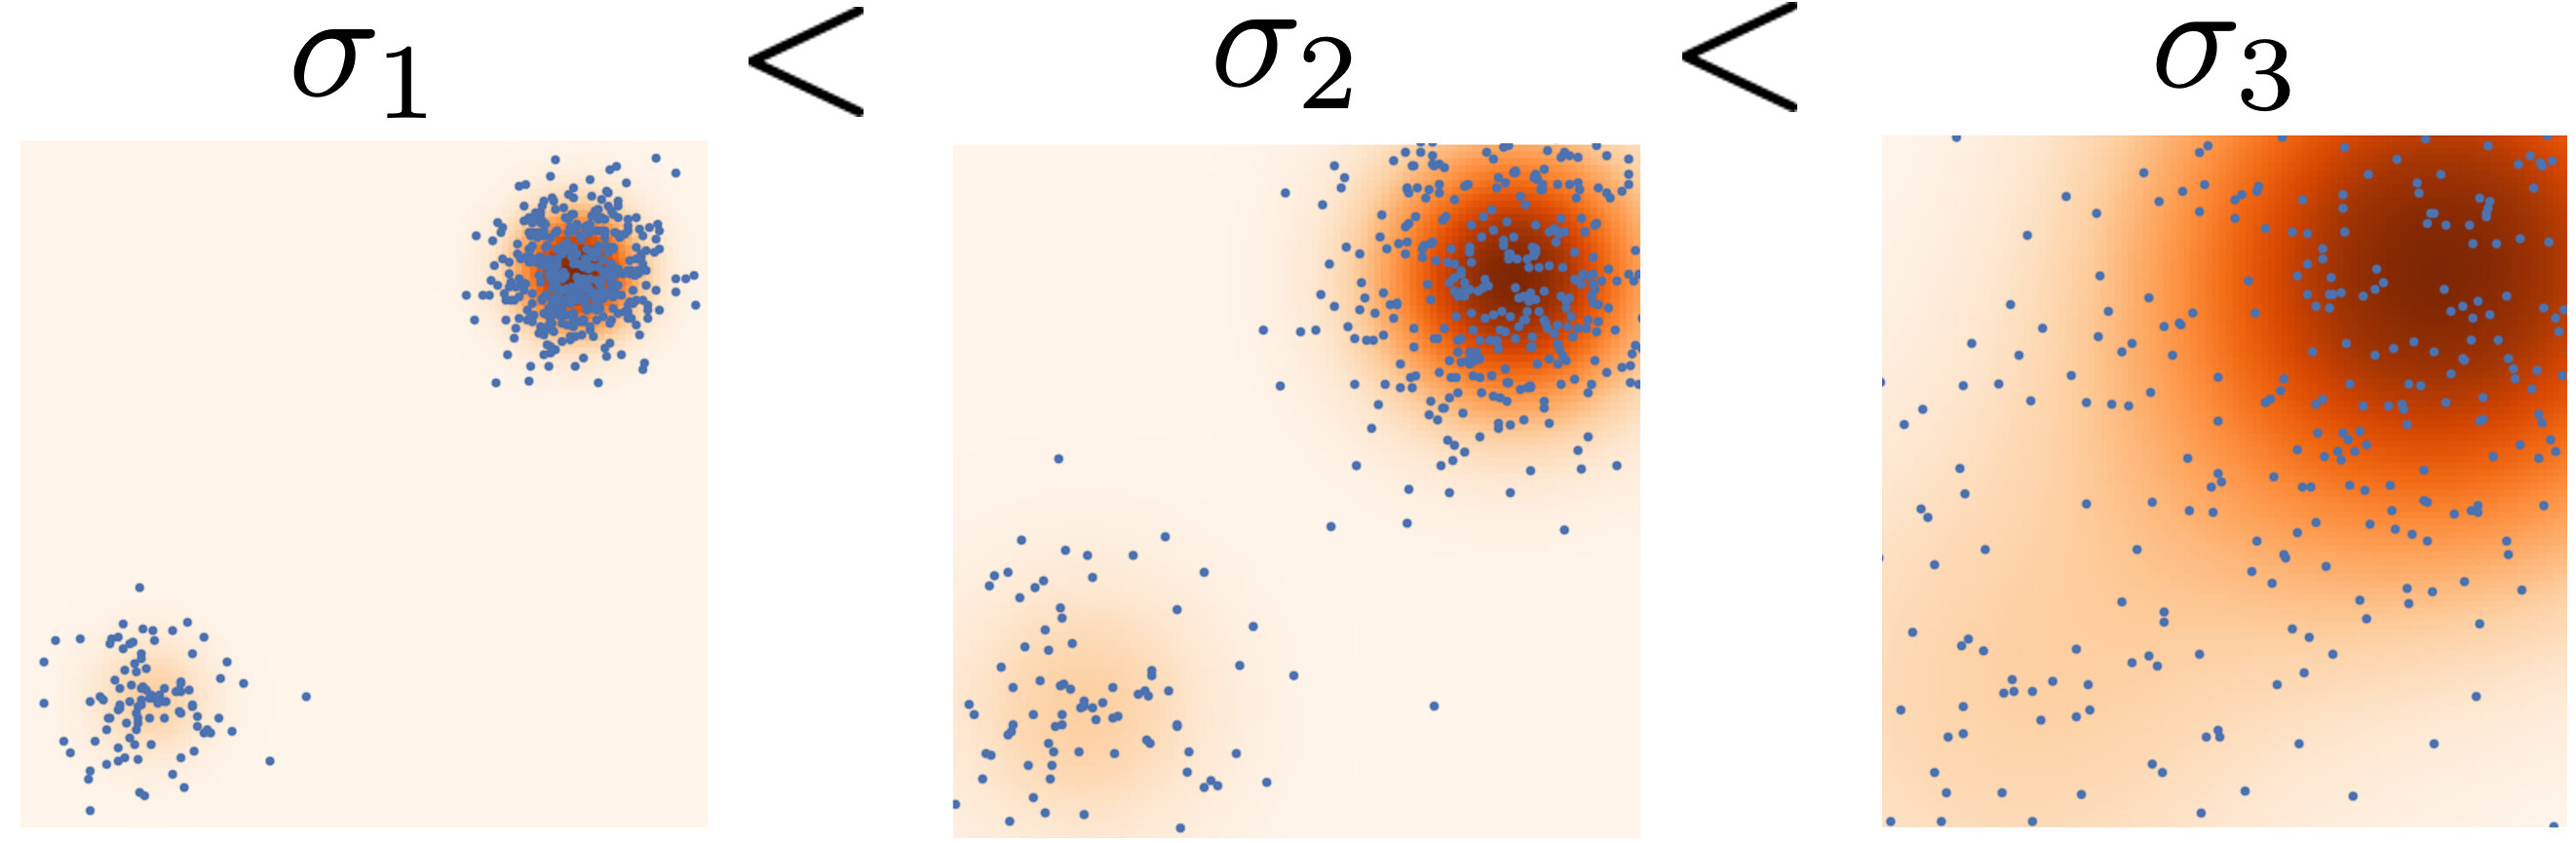
\includegraphics[width=0.55\linewidth]{figs/multi_scale}
    \end{figure}
    \vspace{-0.3cm}
    \begin{figure}
        
\includegraphics[width=\linewidth]{figs/duoduo}
    \end{figure}
\end{frame}
%=======
\begin{frame}{Recap of Previous Lecture}
    \myfootnotewithlink{https://arxiv.org/abs/2006.09011}{Song Y. et al. Improved Techniques for Training Score-Based Generative Models, 2020}
    \begin{block}{NCSN Training}
        \begin{enumerate}
            \item Obtain a sample $\bx_0 \sim \pd(\bx)$.
            \item Sample noise level $t \sim U\{1, T\}$ and noise $\bepsilon \sim \cN(0, \bI)$.
            \item Construct noisy image $\bx_t = \bx_0 + \sigma_t \cdot \bepsilon$.
            \item Compute the loss $ \cL = \sigma_t^2 \cdot \| \bs_{\btheta, \sigma_t}(\bx_t) + \frac{\bepsilon}{\sigma_t} \|^2 $.
        \end{enumerate}
    \end{block}
    \begin{block}{NCSN Sampling (Annealed Langevin Dynamics)}
        \begin{itemize}
            \item Sample $\bx_0 \sim \cN(0, \sigma_T^2 \cdot \bI) \approx q(\bx_T)$.
            \item Apply $L$ steps of Langevin dynamics:
            \vspace{-0.2cm}
            \[
                \bx_l = \bx_{l-1} + \frac{\eta_t}{2} \cdot \bs_{\btheta, \sigma_t}(\bx_{l - 1}) + \sqrt{\eta_t} \cdot \bepsilon_l.
            \] 
            \vspace{-0.5cm}
            \item Update $\bx_0 := \bx_L$ and proceed to the next $\sigma_t$.
        \end{itemize}
    \end{block}
\end{frame}
%=======
\begin{frame}{Recap of Previous Lecture}
    \myfootnotewithlink{https://arxiv.org/abs/2403.18103}{Chan S. Tutorial on Diffusion Models for Imaging and Vision, 2024}
    \begin{block}{Forward Gaussian Diffusion Process}
        Let $\bx_0 = \bx \sim \pd(\bx)$, $\beta_t \ll 1$, $\alpha_t = 1 - \beta_t$ and $\bar{\alpha}_t = \prod_{s=1}^t \alpha_s$. 
        \begin{align*}
            \bx_t &= \sqrt{1 - \beta_t} \cdot \bx_{t - 1} + \sqrt{\beta_t} \cdot \bepsilon, \quad \text{where }\bepsilon \sim \cN(0, \bI); \\
            \bx_t &= \sqrt{\bar{\alpha}_t} \cdot \bx_{0} + \sqrt{1 - \bar{\alpha}_t} \cdot \bepsilon, \quad \text{where } \bepsilon \sim \cN(0, \bI).
        \end{align*}
        \vspace{-0.6cm}
        \begin{align*}
            q(\bx_t | \bx_{t-1}) &= \cN(\sqrt{1 - \beta_t} \cdot \bx_{t-1}, \beta_t \cdot \bI); \\
            q(\bx_t | \bx_0) &= \cN(\sqrt{\bar{\alpha}_t} \cdot \bx_0, (1 - \bar{\alpha}_t) \cdot \bI).
        \end{align*}
        \vspace{-0.6cm}
    \end{block}
    \begin{figure}
        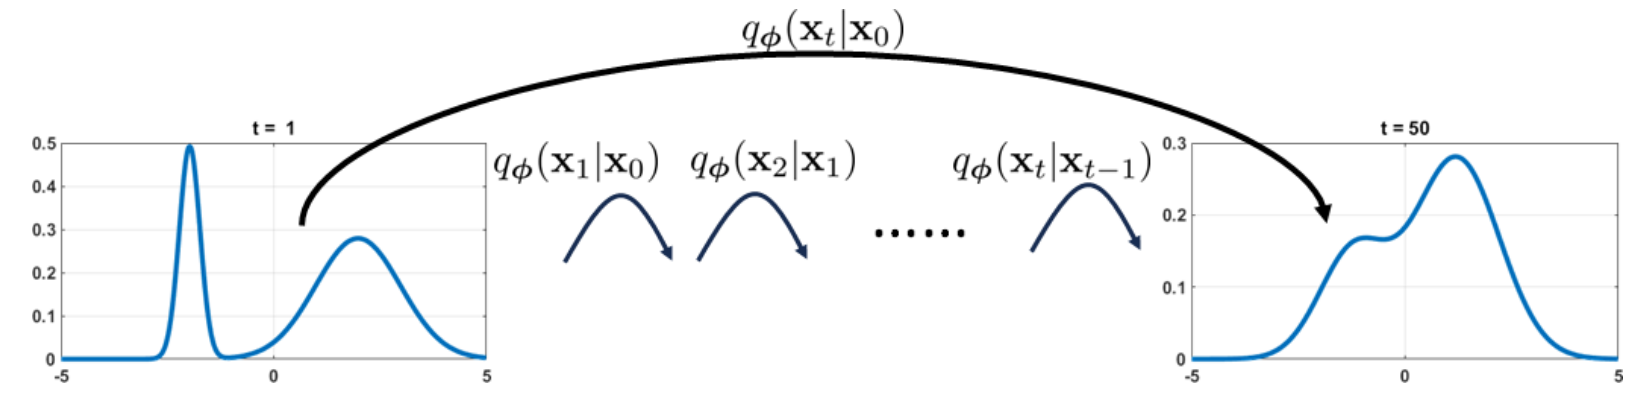
\includegraphics[width=0.8\linewidth]{figs/conditional_diffusion}
    \end{figure}
\end{frame}
%=======
\begin{frame}{Recap of Previous Lecture}
    \myfootnotewithlink{https://ayandas.me/blog-tut/2021/12/04/diffusion-prob-models.html}{Das A. An Introduction to Diffusion Probabilistic Models, blog post, 2021}
    \textbf{Diffusion} describes the process where particles migrate from regions of high density to regions of low density.
    \vspace{-0.2cm}
    \begin{figure}
        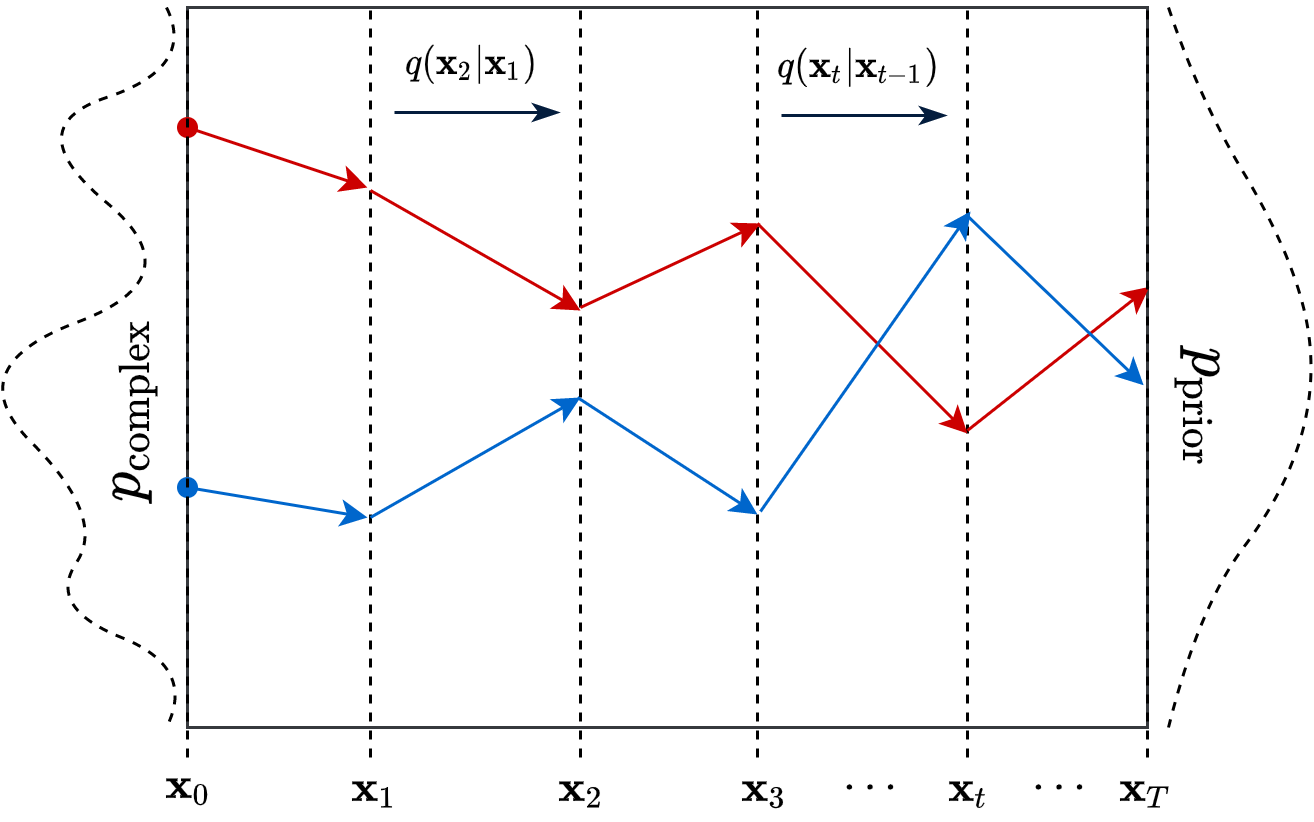
\includegraphics[width=0.5\linewidth]{figs/diffusion_over_time}
    \end{figure}
    \vspace{-0.6cm}
    \begin{enumerate}
        \item $\bx_0 = \bx \sim \pd(\bx)$;
        \item $\bx_t = \sqrt{1 - \beta_t} \cdot \bx_{t - 1} + \sqrt{\beta_t} \cdot \bepsilon$, with $\bepsilon \sim \cN(0, \bI)$, $t \geq 1$;
        \item $\bx_T \sim p_{\infty}(\bx) = \cN(0, \bI)$, for $T \gg 1$.
    \end{enumerate}
    If we can invert this process, we would have a way to sample $\bx \sim \pd(\bx)$ using noise samples, i.e. $p_{\infty}(\bx) = \cN(0, \bI)$. \\ 
    Hence, our objective becomes to reverse this process.
\end{frame}
%=======
\begin{frame}{Recap of Previous Lecture}
    \myfootnotewithlink{https://lilianweng.github.io/posts/2021-07-11-diffusion-models/}{Weng L. What are Diffusion Models?, blog post, 2021}
    \vspace{-0.3cm}
    \begin{figure}
        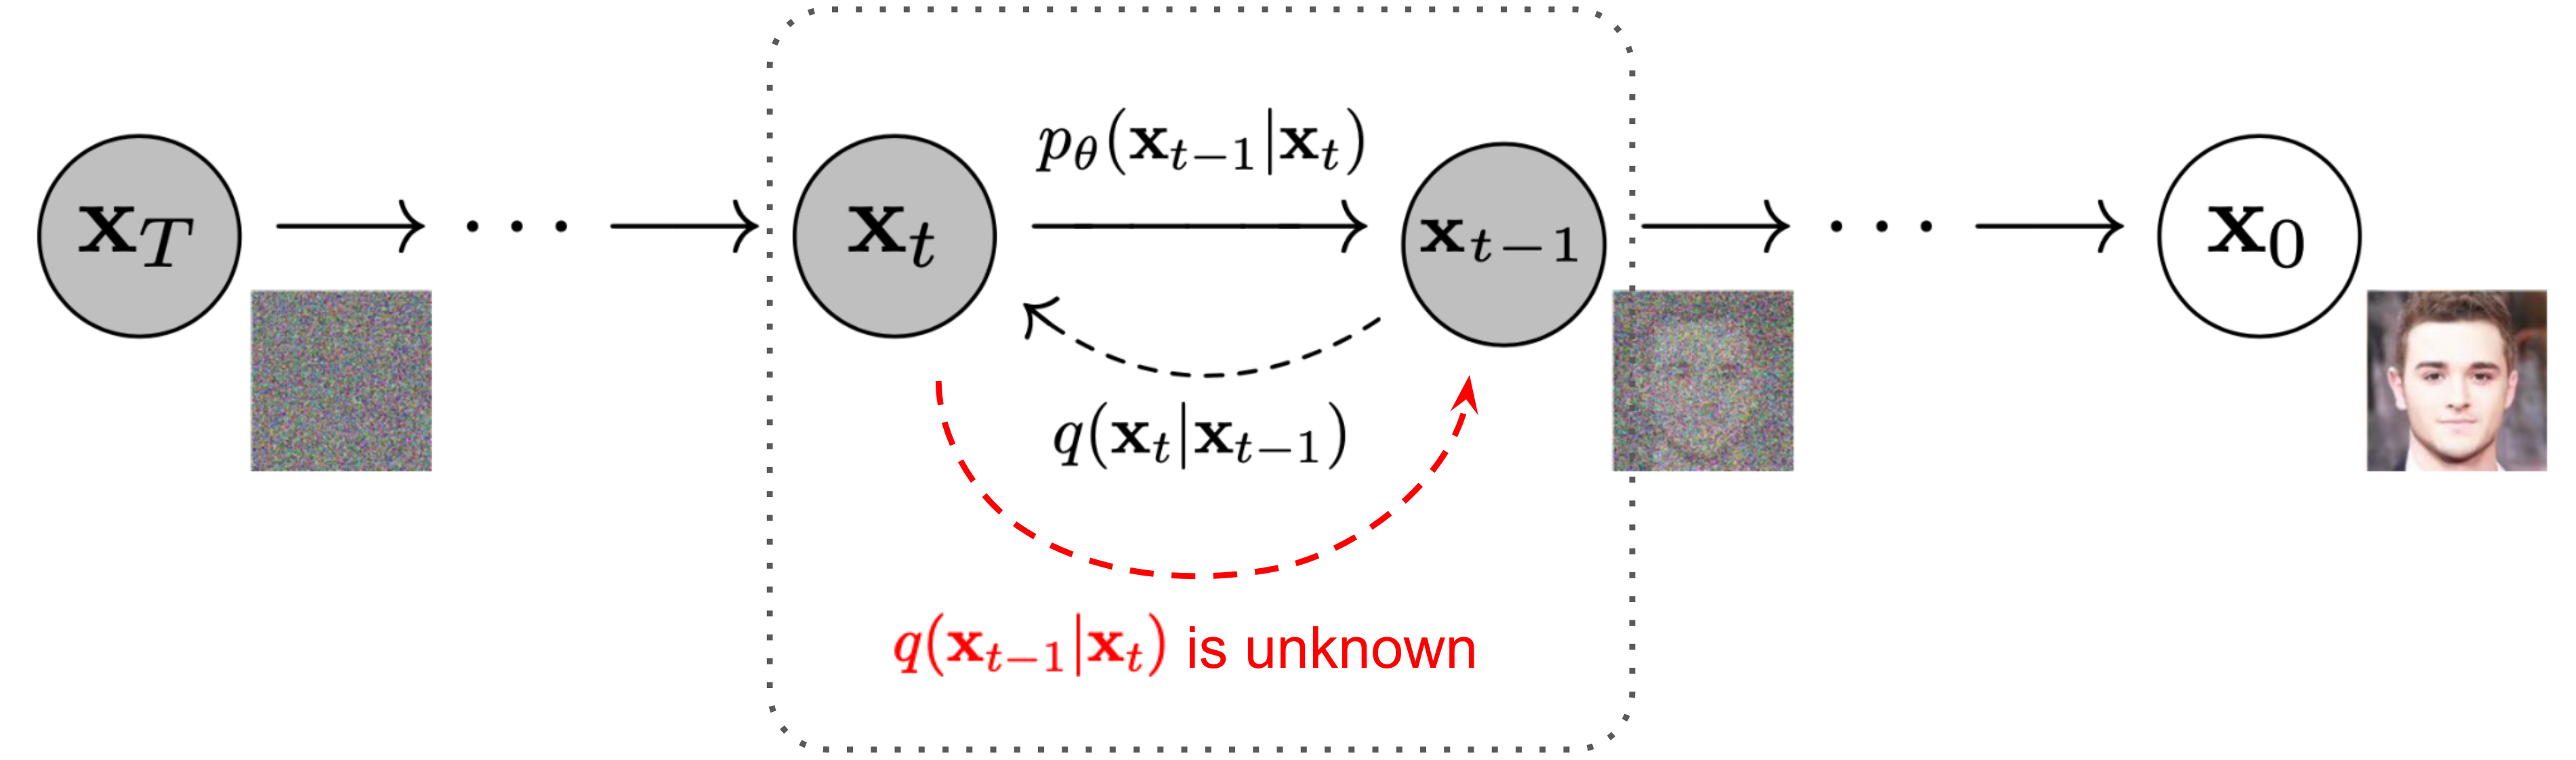
\includegraphics[width=0.8\linewidth]{figs/DDPM}
    \end{figure}
    \vspace{-0.5cm}
    \begin{block}{Reverse Process (Ancestral Sampling)}
        \vspace{-0.5cm}
        {\small
        \[
            q(\bx_{t-1}|\bx_{t}) = \frac{q(\bx_{t}|\bx_{t-1}) {\color{violet}q(\bx_{t-1})}}{{\color{violet}q(\bx_{t})}} \approx \pt(\bx_{t - 1} | \bx_t) = \cN \left(\bmu_{\btheta, t}(\bx_t), \bsigma_{\btheta, t}^2(\bx_t)\right)
        \]}
        {\color{gray}The Feller theorem guarantees this approximation is valid.}
    \end{block}
    \begin{minipage}{0.5\linewidth}
        \begin{block}{Forward Process}
            \begin{enumerate}
                \item $\bx_0 = \bx \sim \pd(\bx)$;
                \item $\bx_t = \sqrt{1 - \beta_t} \cdot \bx_{t - 1} + \sqrt{\beta_t} \cdot \bepsilon$;
                \item $\bx_T \sim p_{\infty}(\bx) = \cN(0, \bI)$.
            \end{enumerate}
        \end{block}
    \end{minipage}%
    \begin{minipage}{0.55\linewidth}
        \begin{block}{Reverse Process}
            \begin{enumerate}
                \item $\bx_T \sim p_{\infty}(\bx) = \cN(0, \bI)$;
                \item $\bx_{t - 1} = \bsigma_{\btheta, t}(\bx_t) \cdot \bepsilon + \bmu_{\btheta, t}(\bx_t)$;
                \item $\bx_0 = \bx \sim \pd(\bx)$;
            \end{enumerate}
        \end{block}
    \end{minipage}
\end{frame}
%=======
\begin{frame}{Outline}
    \tableofcontents
\end{frame}
%=======
\section{Denoising Diffusion Probabilistic Model (DDPM)}
%=======
\begin{frame}{Conditioned Reverse Distribution}
    \myfootnotewithlink{https://arxiv.org/abs/2006.11239}{Ho J. Denoising Diffusion Probabilistic Models, 2020}
    \begin{block}{Reverse Kernel (\textbf{Intractable})}
        \vspace{-0.3cm}
        \[
            q(\bx_{t-1}|\bx_{t}) = \frac{q(\bx_{t}|\bx_{t-1}) {\color{violet}q(\bx_{t-1})}}{{\color{violet}q(\bx_{t})}} 
        \]
        \vspace{-0.5cm}
    \end{block}
    \eqpause
    \begin{block}{Conditioned Reverse Kernel (\textbf{Tractable})}
        \vspace{-0.6cm}
        \begin{align*}
            q(\bx_{t-1}|\bx_{t}, {\color{olive}\bx_0}) & = \frac{q(\bx_{t}|\bx_{t-1}, {\color{olive}\bx_0}) q(\bx_{t-1} | {\color{olive}\bx_0}) }{q(\bx_{t}| {\color{olive}\bx_0})} \\
            \nextonslide{& = \frac{\cN(\sqrt{1 - \beta_t} \cdot \bx_{t-1}, \beta_t \bI) \cdot \cN(\sqrt{\bar{\alpha}_{t-1}} \cdot \bx_0, (1 - \bar{\alpha}_{t-1}) \cdot \bI)}{ \cN(\sqrt{\bar{\alpha}_t} \cdot \bx_0, (1 - \bar{\alpha}_t) \cdot \bI)}} \\
            \nextonslide{&= \cN(\tilde{\bmu}_t(\bx_t, \bx_0), \tilde{\beta}_t \cdot \bI)}
        \end{align*}
        \vspace{-0.7cm}
    \end{block}
    Here,
    \begin{align*}
        \tilde{\bmu}_t(\bx_t, \bx_0) &= \frac{\sqrt{\alpha_t}(1 - \bar{\alpha}_{t-1})}{1 - \bar{\alpha}_t} \cdot \bx_t + \frac{\sqrt{\bar{\alpha}_{t-1}}(1 - \alpha_t)}{1 - \bar{\alpha}_t} \cdot \bx_0; \\
        \tilde{\beta}_t &= \frac{(1 - \alpha_t)(1 - \bar{\alpha}_{t-1})}{1 - \bar{\alpha}_t} = \text{const}.
    \end{align*}
\end{frame}
%=======
\begin{frame}{Distribution Summary}
    \myfootnotewithlink{https://arxiv.org/abs/2006.11239}{Ho J. Denoising Diffusion Probabilistic Models, 2020}

    \textbf{Forward process} maps any distribution $\pd(\bx)$ to $\cN(0, \bI)$ by injection of noise:
    \begin{align*}
        q(\bx_t | \bx_{t-1}) &= \cN(\sqrt{1 - \beta_t} \cdot \bx_{t-1}, \beta_t \cdot \bI); \\
        q(\bx_t | \bx_0) &= \cN(\sqrt{\bar{\alpha}_t} \cdot \bx_0, (1 - \bar{\alpha}_t) \cdot \bI).
    \end{align*}
    \eqpause
    \textbf{Reverse process} refers to an intractable distribution that can be approximated by a normal distribution (with unknown parameters) for small $\beta_t$:
    \[
        q(\bx_{t-1}|\bx_{t}) = \frac{q(\bx_{t}|\bx_{t-1}) q(\bx_{t-1})}{q(\bx_{t})} \approx \cN \left(\bmu_{\btheta, t}(\bx_t), \bsigma_{\btheta, t}^2(\bx_t)\right)
    \]
    \eqpause
    \textbf{Conditioned reverse process} is a normal distribution with known parameters, describing how to denoise a noisy image $\bx_t$ when we know the clean image $\bx_0$.
    \[
        q(\bx_{t-1}|\bx_{t}, {\color{olive}\bx_0}) = \cN(\tilde{\bmu}_t(\bx_t, \bx_0), \tilde{\beta}_t \cdot \bI)
    \]
\end{frame}
%=======
\subsection{Gaussian Diffusion Model as VAE}
%=======
\begin{frame}{Gaussian Diffusion Model as VAE}
    \myfootnotewithlink{https://ayandas.me/blog-tut/2021/12/04/diffusion-prob-models.html}{Das A. An Introduction to Diffusion Probabilistic Models, blog post, 2021}
    Let's treat $\bz = (\bx_1, \dots, \bx_T)$ as a latent variable (\textbf{note:} each $\bx_t$ has the same dimension), and $\bx = \bx_0$ as the observed variable.
    \begin{block}{Latent Variable Model}
        \vspace{-0.3cm}
        \[
            \pt(\bx, \bz) = \pt(\bx | \bz) \pt(\bz)
        \]    
        \vspace{-0.7cm}
    \end{block}
    \eqpause
    \begin{figure}
        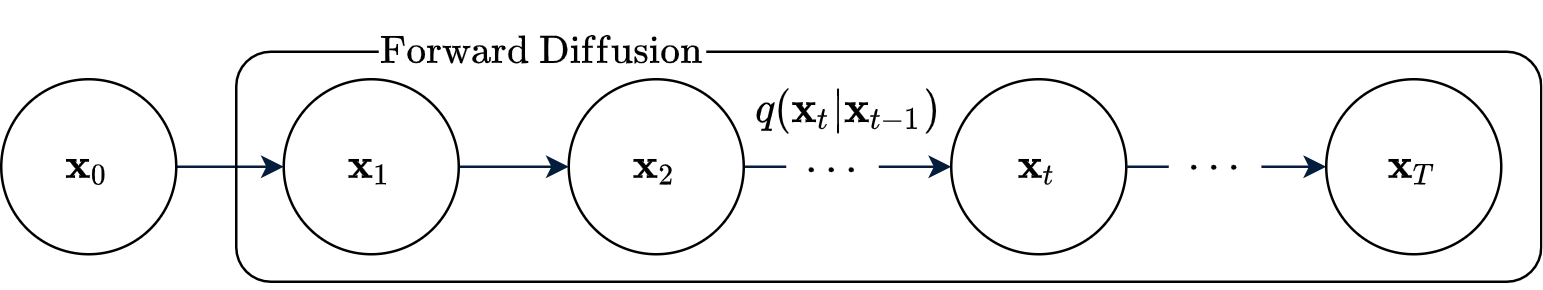
\includegraphics[width=0.8\linewidth]{figs/diffusion_pgm_forward}
    \end{figure}
    \eqpause
    \vspace{-0.3cm}
    \begin{block}{Forward Diffusion}
        \begin{itemize}
            \item Variational posterior distribution (encoder)
            \vspace{-0.3cm}
            \[
                q(\bz | \bx) = q(\bx_1, \dots, \bx_T | \bx_0) = \prod_{t = 1}^T q(\bx_t | \bx_{t - 1}).
            \]
            \item \textbf{Note:} there are no learnable parameters.
        \end{itemize}
        \vspace{-0.5cm}
    \end{block}
\end{frame}
%=======
\begin{frame}{Gaussian Diffusion Model as VAE}
    \myfootnotewithlink{https://ayandas.me/blog-tut/2021/12/04/diffusion-prob-models.html}{Das A. An Introduction to Diffusion Probabilistic Models, blog post, 2021}
    \[
        \pt(\bx, \bz) = \pt(\bx | \bz) \pt(\bz)
    \]    
    \eqpause
    \vspace{-0.5cm}
    \begin{figure}
        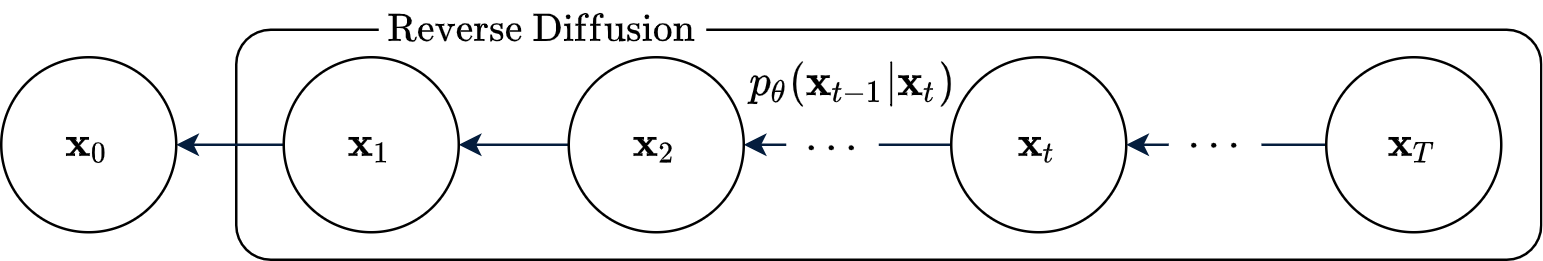
\includegraphics[width=0.8\linewidth]{figs/diffusion_pgm_reverse}
    \end{figure}
    \eqpause
    \vspace{-0.2cm}
    \begin{block}{Reverse Diffusion}
        \begin{itemize}
            \item Generative distribution (decoder)
            \[
                \pt(\bx | \bz) = \pt(\bx_0 | \bx_1).
            \]
            \vspace{-0.7cm}
            \eqpause
            \item Prior distribution
            \vspace{-0.3cm}
            \[
                \pt(\bz) = \pt(\bx_1, \dots, \bx_T) = \prod_{t=2}^T \pt(\bx_{t - 1} | \bx_t)  \cdot p(\bx_T).
            \]
            \vspace{-0.3cm}
        \end{itemize}
        \eqpause
        \textbf{Note:} This differs from the vanilla VAE due to the complex decoder $\pt(\bx | \bz)$ and the standard normal prior $p(\bz)$.
    \end{block}
\end{frame}
%=======
\subsection{ELBO Derivation}
%=======
\begin{frame}{ELBO for Gaussian Diffusion Model}
    \myfootnotewithlink{https://arxiv.org/abs/2006.11239}{Ho J. Denoising Diffusion Probabilistic Models, 2020}
    \begin{block}{Standard ELBO}
        \vspace{-0.3cm}
        \[
            \log \pt(\bx) \geq \bbE_{q({\color{teal}\bz} | \bx)} \log \frac{\pt(\bx, {\color{teal}\bz})}{q({\color{teal}\bz} | \bx)} = \cL_{\bphi, \btheta}(\bx) \rightarrow \max_{q, \btheta}
        \]
        \vspace{-0.5cm}
    \end{block}
    \eqpause
    \begin{block}{Derivation}
        \vspace{-0.5cm}
        \begin{align*}
            \cL_{\bphi, \btheta}(\bx) &= \bbE_{q({\color{teal}\bx_{1:T}} | \bx_0)} \log \frac{\pt(\bx_0, {\color{teal}\bx_{1:T}})}{q({\color{teal}\bx_{1:T}} | \bx_0)} \\
            \nextonslide{& = \bbE_{q(\bx_{1:T} | \bx_0)} \log \frac{p(\bx_T) \prod_{t=1}^T \pt(\bx_{t-1} | \bx_t) }{\prod_{t=1}^T {\color{violet}q(\bx_t | \bx_{t-1})}}}
        \end{align*}
        \vspace{-0.3cm}
        \eqpause
        \begin{itemize}
            \item Let's try to decompose the ELBO into individual KL divergence terms.
            \item We need to replace $q(\bx_t | \bx_{t - 1})$ with $q(\bx_{t - 1} | \bx_t)$ in the denominator.
            \item Let's condition on $\bx_0$ to make the reverse $q(\bx_{t - 1} | \bx_t)$ tractable.
        \end{itemize}
    \end{block}
\end{frame}
%=======
\begin{frame}{ELBO for Gaussian Diffusion Model}
    \myfootnotewithlink{https://arxiv.org/abs/2006.11239}{Ho J. Denoising Diffusion Probabilistic Models, 2020}
    \[
         {\color{teal}q(\bx_t | \bx_{t-1}, \bx_0)}  = \frac{q(\bx_{t-1}|\bx_t, \bx_0)q(\bx_{t} | \bx_0)}{q(\bx_{t-1}| \bx_0)}
    \]
    \eqpause
    \vspace{-0.3cm}
    \begin{block}{Derivation (continued)}
        \vspace{-0.6cm}
        {\small
        \begin{align*}
            \cL_{\bphi, \btheta}(\bx) & = \bbE_{q(\bx_{1:T} | \bx_0)} \log \frac{p(\bx_T) \prod_{t=1}^T \pt(\bx_{t-1} | \bx_t) }{\prod_{t=1}^T {\color{violet}q(\bx_t | \bx_{t-1})}}  \\ 
            \nextonslide{& = \bbE_{q(\bx_{1:T} | \bx_0)} \log \frac{p(\bx_T) \prod_{t=1}^T \pt(\bx_{t-1} | \bx_t) }{\prod_{t=1}^T q(\bx_t | \bx_{t-1}, {\color{olive}\bx_0})}  }\\ 
            \nextonslide{& = \bbE_{q(\bx_{1:T} | \bx_0)} \log \frac{p(\bx_T) \pt(\bx_0 | \bx_1) \prod_{t=2}^T \pt(\bx_{t-1} | \bx_t) }{q(\bx_1 | \bx_0)\prod_{t=2}^T {\color{teal}q(\bx_t | \bx_{t-1}, \bx_0)}} }\\
            \nextonslide{& = \bbE_{q(\bx_{1:T} | \bx_0)} \log \frac{p(\bx_T) \pt(\bx_0 | \bx_1) \prod_{t=2}^T \pt(\bx_{t-1} | \bx_t) }{{\color{violet}q(\bx_1 | \bx_0)}\prod_{t=2}^T \frac{q(\bx_{t-1}|\bx_t, \bx_0) {\color{violet}q(\bx_{t} | \bx_0)}}{{\color{violet}q(\bx_{t-1}| \bx_0)}}} }\\
            \nextonslide{& = \bbE_{q(\bx_{1:T} | \bx_0)} \log \frac{{\color{violet}p(\bx_T)} {\color{olive}\pt(\bx_0 | \bx_1)} \prod_{t=2}^T \pt(\bx_{t-1} | \bx_t) }{{\color{violet}q(\bx_T | \bx_0)}\prod_{t=2}^T q(\bx_{t-1}|\bx_t, \bx_0)} }
        \end{align*}}
    \end{block}
\end{frame}
%=======
\begin{frame}{ELBO for Gaussian Diffusion Model}
    \myfootnotewithlink{https://arxiv.org/abs/2006.11239}{Ho J. Denoising Diffusion Probabilistic Models, 2020}
    \begin{block}{Derivation (continued)}
        \vspace{-0.7cm}
        {\small
        \begin{multline*}
            \cL_{\bphi, \btheta}(\bx) = \bbE_{q(\bx_{1:T} | \bx_0)} \log \frac{{\color{violet}p(\bx_T)} {\color{olive}\pt(\bx_0 | \bx_1)} \prod_{t=2}^T \pt(\bx_{t-1} | \bx_t) }{{\color{violet}q(\bx_T | \bx_0)}\prod_{t=2}^T q(\bx_{t-1}|\bx_t, \bx_0)} 
            \nextonslide{ = \\ = \bbE_{{\color{teal}q(\bx_{1:T} | \bx_0)}} \biggl[ \log {\color{olive}\pt(\bx_0 | \bx_1)} + \log {\color{violet}\frac{p(\bx_T)}{q(\bx_T | \bx_0)}} + \sum_{t=2}^T \log \left( \frac{\pt(\bx_{t-1} | \bx_t)}{q(\bx_{t-1}|\bx_{t}, \bx_0)}\right) \biggr] }
            \nextonslide{= \\ = \bbE_{{\color{teal}q(\bx_1 | \bx_0)}} \log \pt(\bx_0 | \bx_1) + \bbE_{{\color{teal}q(\bx_T | \bx_0)}} \log \frac{p(\bx_T)}{q(\bx_T | \bx_0)} + \\
             + \sum_{t=2}^T \bbE_{{\color{teal}q(\bx_{t-1}, \bx_t | \bx_0)}} \log \left( \frac{\pt(\bx_{t-1} | \bx_t)}{q(\bx_{t-1}|\bx_{t}, \bx_0)}\right) \biggr] }
            \nextonslide{= \\ = \bbE_{q(\bx_1 | \bx_0)} \log \pt(\bx_0 | \bx_1) - \KL\bigl(q(\bx_T | \bx_0) \| p(\bx_T)\bigr) - \\
            - \sum_{t=2}^T \underbrace{ \bbE_{q(\bx_t | \bx_0)} \KL \bigl(q(\bx_{t-1} | \bx_t, \bx_0) \| \pt(\bx_{t-1} | \bx_t)\bigr)}_{\cL_t}}
        \end{multline*}
        }
        \vspace{-0.3cm}
    \end{block}
\end{frame}
%=======
\begin{frame}{ELBO for Gaussian Diffusion Model}
    \myfootnotewithlink{https://arxiv.org/abs/2006.11239}{Ho J. Denoising Diffusion Probabilistic Models, 2020}
        \vspace{-0.5cm}
        \begin{multline*}
            \cL_{\bphi, \btheta}(\bx) =  {\color{olive}\bbE_{q(\bx_1 | \bx_0)} \log \pt(\bx_0 | \bx_1)} - {\color{violet}\KL\bigl(q(\bx_T | \bx_0) \| p(\bx_T)\bigr)} - \\
            - {\color{teal}\sum_{t=2}^T \underbrace{ \bbE_{q(\bx_t | \bx_0)} \KL \bigl(q(\bx_{t-1} | \bx_t, \bx_0) \| \pt(\bx_{t-1} | \bx_t)\bigr)}_{\cL_t}}
        \end{multline*}
        \vspace{-0.5cm}
    \eqpause
    \begin{itemize}
        \item {\color{olive}First term} is the decoder distribution
        \[
            \log \pt(\bx_0 | \bx_1) = \log \cN \bigl(\bx_0 | \bmu_{\btheta, t}(\bx_1), \bsigma_{\btheta, t}^2(\bx_1)\bigr),
        \] 
        with $\bx_1 \sim q(\bx_1 | \bx_0)$.
        \eqpause
        \item {\color{violet}Second term} is constant: 
        \begin{itemize}
            \item $p(\bx_T) = \cN(0, \bI)$;
            \item $q(\bx_T | \bx_0) = \cN(\sqrt{\bar{\alpha}_T} \cdot \bx_0, (1 - \bar{\alpha}_T) \cdot \bI)$.
        \end{itemize}
        \eqpause
        \item {\color{teal}Third term} is the main contributor to the ELBO.
    \end{itemize}
\end{frame}
%=======
\begin{frame}{ELBO for Gaussian Diffusion Model}
    \myfootnotewithlink{https://arxiv.org/abs/2208.11970}{Luo C. Understanding Diffusion Models: A Unified Perspective, 2022}
    \begin{figure}
        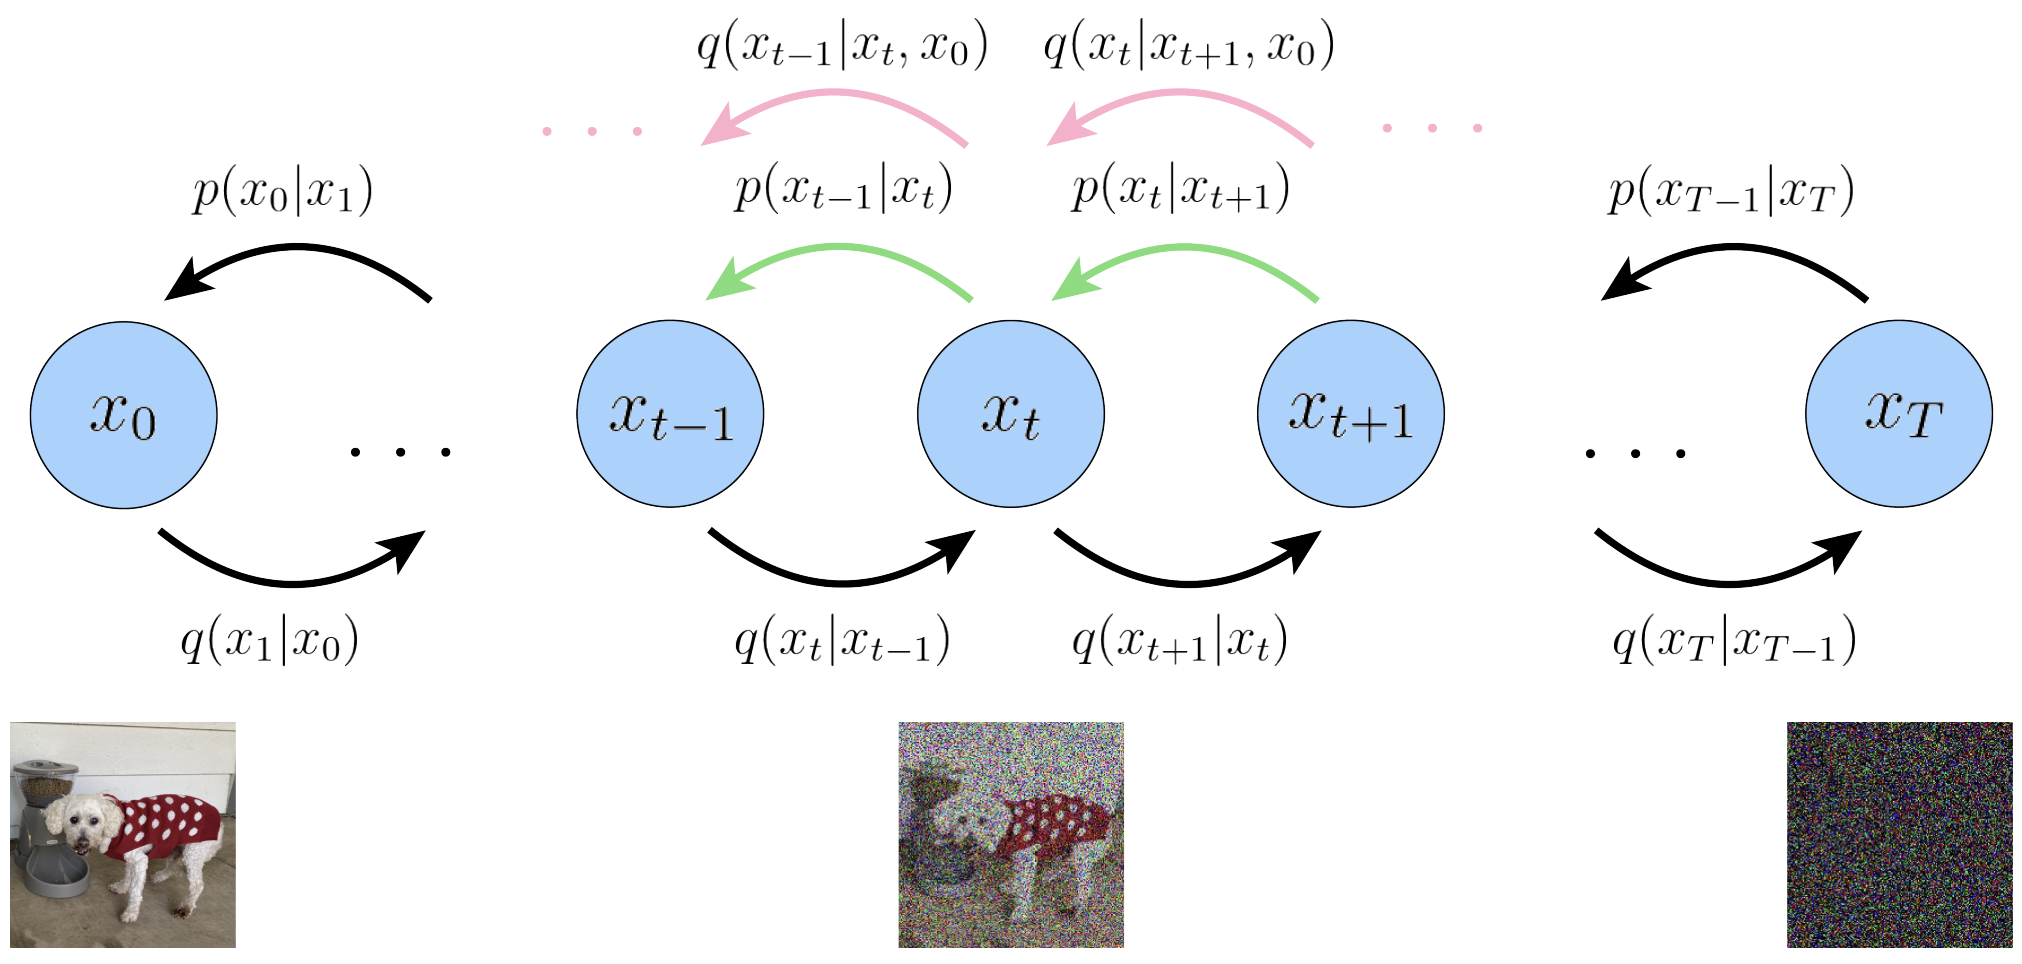
\includegraphics[width=\linewidth]{figs/diffusion_objective}
    \end{figure}
    \[
        \cL_t = \bbE_{q(\bx_t | \bx_0)} \KL \bigl(q(\bx_{t-1} | \bx_t, \bx_0) \| \pt(\bx_{t-1} | \bx_t)\bigr)
    \]
    \begin{align*}
        q(\bx_{t-1} | \bx_t, \bx_0) &= \cN(\bx_{t-1} | \tilde{\bmu}_t(\bx_t, \bx_0), \tilde{\beta}_t \bI), \\
        \pt(\bx_{t - 1} | \bx_t) &= \cN \bigl(\bx_{t - 1} | \bmu_{\btheta, t}(\bx_t), \bsigma_{\btheta, t}^2(\bx_t)\bigr)
    \end{align*}
\end{frame}
%=======
\begin{frame}{ELBO for Gaussian Diffusion Model}
    \myfootnotewithlink{https://arxiv.org/abs/2006.11239}{Ho J. Denoising Diffusion Probabilistic Models, 2020}
    \[
        \cL_t = \bbE_{q(\bx_t | \bx_0)} \KL \bigl(q(\bx_{t-1} | \bx_t, \bx_0) \| \pt(\bx_{t-1} | \bx_t)\bigr)
    \]
    \vspace{-0.7cm}
    \begin{align*}
        q(\bx_{t-1} | \bx_t, \bx_0) &= \cN(\bx_{t-1} | \tilde{\bmu}_t(\bx_t, \bx_0), \tilde{\beta}_t \bI), \\
        \pt(\bx_{t - 1} | \bx_t) &= \cN \bigl(\bx_{t - 1} | \bmu_{\btheta, t}(\bx_t), {\color{violet}\bsigma_{\btheta, t}^2(\bx_t)}\bigr)
    \end{align*}
    \eqpause
    Let's assume that
    \[
        {\color{violet}\bsigma_{\btheta, t}^2(\bx_t) = \tilde{\beta}_t \bI} \quad \Rightarrow \quad \pt(\bx_{t - 1} | \bx_t) = \cN \bigl(\bx_{t - 1} | \bmu_{\btheta, t}(\bx_t), {\color{violet}\tilde{\beta}_t \bI} \bigr).
    \]
    \eqpause
    Theoretically, the optimal $\bsigma_{\btheta, t}^2(\bx_t)$ lies in $[\tilde{\beta}_t, \beta_t]$:
    \begin{itemize}
        \item $\beta_t$ is optimal for $\bx_0 \sim \cN(0, \bI)$;
        \item $\tilde{\beta}_t$ is optimal for $\bx_0 \sim \delta(\bx_0 - \bx^*)$.
    \end{itemize}
    \eqpause
    \begin{align*}
        \cL_t &= \bbE_{q(\bx_t | \bx_0)} KL\Bigl(\cN\bigl(\tilde{\bmu}_t(\bx_t, \bx_0), \tilde{\beta}_t \bI \bigr) \| \cN\bigl(\bmu_{\btheta, t}(\bx_t), \tilde{\beta}_t \bI\bigr)\Bigr) \\ 
        \nextonslide{&= \bbE_{q(\bx_t | \bx_0)} \left[\frac{1}{2\tilde{\beta}_t} \bigl\| \tilde{\bmu}_t(\bx_t, \bx_0) - \bmu_{\btheta, t}(\bx_t) \bigr\|^2  \right]}
    \end{align*}
\end{frame}
%=======
\begin{frame}{ELBO for Gaussian Diffusion Model}
    \myfootnotewithlink{https://arxiv.org/abs/2006.11239}{Ho J. Denoising Diffusion Probabilistic Models, 2020}
    \begin{block}{Training}
        \begin{enumerate}
            \item Obtain a sample $\bx_0 \sim \pd(\bx)$.
            \item Generate a noisy image $\bx_t = \sqrt{\bar{\alpha}_t} \cdot \bx_0 + \sqrt{1 - \bar{\alpha}_t} \cdot \bepsilon$, with $\bepsilon \sim \cN(0, \bI)$.
            \item Compute the ELBO
            \vspace{-0.3cm}
            \begin{multline*}
                \cL_{\bphi, \btheta}(\bx) =  {\color{olive}\bbE_{q(\bx_1 | \bx_0)} \log \pt(\bx_0 | \bx_1)} - {\color{violet}\KL\bigl(q(\bx_T | \bx_0) \| p(\bx_T)\bigr)} - \\
                - {\color{teal}\sum_{t=2}^T \underbrace{ \bbE_{q(\bx_t | \bx_0)} \left[\frac{1}{2\tilde{\beta}_t} \bigl\| \tilde{\bmu}_t(\bx_t, \bx_0) - \bmu_{\btheta, t}(\bx_t) \bigr\|^2  \right]}_{\cL_t}}
            \end{multline*}
            \vspace{-0.7cm}
        \end{enumerate}
    \end{block}
    \eqpause
    \begin{block}{Sampling}
        \begin{enumerate}
            \item Sample $\bx_T \sim \cN(0, \bI)$.
            \item Denoise: $\bx_{t - 1} = \bmu_{\btheta, t}(\bx_t) +  \sqrt{\tilde{\beta}_t} \cdot \bepsilon$, $\bepsilon \sim \cN(0, \bI)$.
        \end{enumerate}
    \end{block}
\end{frame}
%=======
\subsection{Reparametrization}
%=======
\begin{frame}{Reparametrization of DDPM}
    \myfootnotewithlink{https://arxiv.org/abs/2006.11239}{Ho J. Denoising Diffusion Probabilistic Models, 2020}
    \[
        \cL_t = \bbE_{q(\bx_t | \bx_0)} \left[\frac{1}{2\tilde{\beta}_t} \bigl\| \tilde{\bmu}_t(\bx_t, \bx_0) - \bmu_{\btheta, t}(\bx_t) \bigr\|^2  \right]
    \]
    \[
        \tilde{\bmu}_t(\bx_t, \bx_0) = \frac{\sqrt{\alpha_t}(1 - \bar{\alpha}_{t-1})}{1 - \bar{\alpha}_t} \cdot \bx_t + \frac{\sqrt{\bar{\alpha}_{t-1}}(1 - \alpha_t)}{1 - \bar{\alpha}_t} \cdot {\color{olive} \bx_0}
    \]
    \eqpause
    \vspace{-0.2cm}
    \[
        \bx_t = \sqrt{\bar{\alpha}_t} \cdot \bx_0 + \sqrt{1 - \bar{\alpha}_t} \cdot \bepsilon \quad \nextonslide{\Rightarrow \quad {\color{olive} \bx_0} = \frac{\bx_t -  \sqrt{1 - \bar{\alpha}_t} \cdot \bepsilon}{\sqrt{\bar{\alpha}_t}}}
    \]
    \eqpause
    \vspace{-0.3cm}
    \begin{itemize}
        \item There is a linear relationship between $\bepsilon$, $\bx_t$, and $\bx_0$.
        \item Let's try to rewrite this mean using only $\bx_t$ and $\bepsilon$.
    \end{itemize}
    \eqpause
    \vspace{-0.2cm}
    \begin{align*}
        \tilde{\bmu}_t(\bx_t, \bepsilon) &= \frac{\sqrt{\alpha_t}(1 - \bar{\alpha}_{t-1})}{1 - \bar{\alpha}_t} \cdot \bx_t + \frac{\sqrt{\bar{\alpha}_{t-1}}(1 - \alpha_t)}{1 - \bar{\alpha}_t} \cdot {\color{olive} \left(\frac{\bx_t -  \sqrt{1 - \bar{\alpha}_t} \cdot \bepsilon}{\sqrt{\bar{\alpha}_t}}\right)} \\
        \nextonslide{&= \frac{1}{\sqrt{\alpha_t}} \cdot \bx_t - \frac{1 - \alpha_t}{\sqrt{\alpha_t (1 - \bar{\alpha}_t)}} \cdot \bepsilon}
    \end{align*}
\end{frame}
%=======
\begin{frame}{Reparametrization of DDPM}
    \myfootnotewithlink{https://arxiv.org/abs/2006.11239}{Ho J. Denoising Diffusion Probabilistic Models, 2020}
    \[
        \cL_t = \bbE_{\color{violet}q(\bx_t | \bx_0)} \left[ {\color{olive}\frac{1}{2\tilde{\beta}_t}} \bigl\| \tilde{\bmu}_t(\bx_t, \bx_0) - \bmu_{\btheta, t}(\bx_t) \bigr\|^2  \right]
    \]
    \vspace{-0.3cm}
    \begin{block}{Reparametrization}
        \vspace{-0.7cm}
        \begin{align*}
            \tilde{\bmu}_t(\bx_t, \bx_0) &= \frac{1}{\sqrt{\alpha_t}} \cdot \bx_t - \frac{1 - \alpha_t}{\sqrt{\alpha_t (1 - \bar{\alpha}_t)}} \cdot \bepsilon \\
            \nextonslide{\bmu_{\btheta, t}(\bx_t) &= \frac{1}{\sqrt{\alpha_t}} \cdot \bx_t - {\color{teal}\frac{1 - \alpha_t}{\sqrt{\alpha_t (1 - \bar{\alpha}_t)}}} \cdot \bepsilon_{\btheta, t}(\bx_t)}
        \end{align*}
        \vspace{-0.7cm}
    \end{block}
    \eqpause
    \vspace{-0.5cm}
    \begin{align*}
        \cL_t &=  \bbE_{\color{violet} \bepsilon \sim \cN(0, \bI)} \left[ \frac{{\color{teal}(1 - \alpha_t)^2}}{{\color{olive}2\tilde{\beta}_t} {\color{teal} \alpha_t (1 - \bar{\alpha}_t)}} \bigl\| \bepsilon - \bepsilon_{\btheta, t}({\color{violet}\bx_t}) \bigr\|^2 \right] \\
        \nextonslide{& =  \bbE_{\color{violet}\bepsilon \sim \cN(0, \bI)} \left[ \frac{(1 - \alpha_t)^2}{2\tilde{\beta}_t \alpha_t (1 - \bar{\alpha}_t)} \Bigl\| \bepsilon - \bepsilon_{\btheta, t}\bigl( {\color{violet}\sqrt{\bar{\alpha}_t} \bx_0 + \sqrt{1 - \bar{\alpha}_t} \bepsilon}\bigr) \Bigr\|^2 \right]}
    \end{align*}
    \eqpause
    At every step of the reverse process, we attempt to predict the noise~$\bepsilon$ that was used in the forward diffusion process!
\end{frame}
%=======
\begin{frame}{Reparametrization of DDPM}
    \myfootnotewithlink{https://arxiv.org/abs/2006.11239}{Ho J. Denoising Diffusion Probabilistic Models, 2020}
    \begin{multline*}
        \cL_{\bphi, \btheta}(\bx) =  {\color{olive}\bbE_{q(\bx_1 | \bx_0)} \log \pt(\bx_0 | \bx_1)} - {\color{violet}\KL\bigl(q(\bx_T | \bx_0) \| p(\bx_T)\bigr)} - \\
        - \sum_{t=2}^T \underbrace{ \bbE_{q(\bx_t | \bx_0)} \KL \bigl(q(\bx_{t-1} | \bx_t, \bx_0) \| \pt(\bx_{t-1} | \bx_t)\bigr)}_{\cL_t}
    \end{multline*}
    \eqpause
    \vspace{-0.3cm}
    \[
        \cL_t  = \bbE_{\bepsilon \sim \cN(0, \bI)} \left[ \frac{(1 - \alpha_t)^2}{2\tilde{\beta}_t \alpha_t (1 - \bar{\alpha}_t)} \Bigl\| \bepsilon - \bepsilon_{\btheta, t}\bigl( \sqrt{\bar{\alpha}_t} \bx_0 + \sqrt{1 - \bar{\alpha}_t} \bepsilon\bigr) \Bigr\|^2 \right]
    \]
    \eqpause
    Let's drop the scaling coefficient.
    \begin{block}{Simplified Objective}
        \vspace{-0.3cm}
        \[
             \cL_{\text{simple}} = \bbE_{t \sim U\{2, T\}} \bbE_{\bepsilon \sim \cN(0, \bI)} \Bigl\| \bepsilon - \bepsilon_{\btheta, t}\bigl( \sqrt{\bar{\alpha}_t} \cdot \bx_0 + \sqrt{1 - \bar{\alpha}_t} \cdot \bepsilon\bigr) \Bigr\|^2 
        \]
    \end{block}
\end{frame}
%=======
\subsection{Overview}
%=======
\begin{frame}{Generative Models Zoo}
    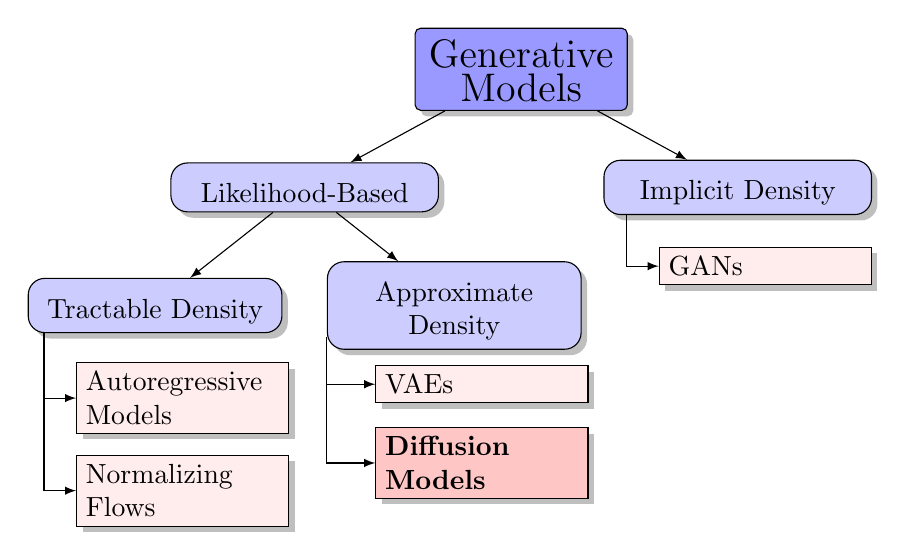
\begin{tikzpicture}[
        basic/.style  = {draw, text width=2cm, drop shadow, rectangle},
        root/.style   = {basic, rounded corners=2pt, thin, text height=1.1em, text width=7em, align=center, fill=blue!40},
        level 1/.style={sibling distance=55mm},
        level 2/.style = {basic, rounded corners=6pt, thin, align=center, fill=blue!20, text height=1.1em, text width=9em, sibling distance=38mm},
        level 3/.style = {basic, rounded corners=6pt, thin,align=center, fill=blue!20, text width=8.5em},
        level 4/.style = {basic, thin, align=left, fill=pink!30, text width=7em},
        level 5/.style = {basic, thin, align=left, fill=pink!90, text width=7em},
        edge from parent/.style={->,draw},
        >=latex]
        
        % root of the the initial tree, level 1
        \node[root] {\Large Generative Models}
        % The first level, as children of the initial tree
        child {node[level 2] (c1) {Likelihood-Based}
            child {node[level 3] (c11) {Tractable Density}}
            child {node[level 3] (c12) {Approximate Density}}
        }
        child {node[level 2] (c2) {Implicit Density}};
        
        % The second level, relatively positioned nodes
        \begin{scope}[every node/.style={level 4}]
            \node [below of = c11, yshift=-5pt, xshift=10pt] (c111) {Autoregressive Models};
            \node [below of = c111, yshift=-5pt] (c112) {Normalizing Flows};
            \node [below of = c12, xshift=10pt] (c121) {VAEs};
            
            \node [below of = c2, xshift=10pt] (c21) {GANs};
        \end{scope}
        
        % The second level, relatively positioned nodes
        \begin{scope}[every node/.style={level 5}]
            \node [below of = c121] (c122) {\textbf{Diffusion \\ Models}};
        \end{scope}
        
        % lines from each level 1 node to every one of its "children"
        \foreach \value in {1,2}
        \draw[->] (c11.194) |- (c11\value.west);
        
        \foreach \value in {1,2}
        \draw[->] (c12.194) |- (c12\value.west);
        
        \draw[->] (c2.194) |- (c21.west);
        
    \end{tikzpicture}
\end{frame}
%=======
\begin{frame}{Denoising Diffusion Probabilistic Model (DDPM)}
    \myfootnotewithlink{https://arxiv.org/abs/2006.11239}{Ho J. Denoising Diffusion Probabilistic Models, 2020}
    \begin{block}{DDPM is a VAE Model}
        \begin{itemize}
            \item The encoder is a fixed Gaussian Markov chain $q(\bx_1, \dots, \bx_T | \bx_0)$.
            \item The latent variable is hierarchical (at each step, its dimension equals the input's).
            \item The decoder is a simple Gaussian model $\pt(\bx_0 | \bx_1)$.
            \item The prior distribution is given by a parametric Gaussian Markov chain $\pt(\bx_{t-1} | \bx_t)$.
        \end{itemize}
    \end{block}
    \eqpause
    \begin{minipage}{0.5\linewidth}
        \begin{block}{Forward Process}
            \begin{enumerate}
                \item $\bx_0 = \bx \sim \pd(\bx)$;
                \item $\bx_t = \sqrt{1 - \beta_t} \cdot \bx_{t - 1} + \sqrt{\beta_t} \cdot \bepsilon$;
                \item $\bx_T \sim p_{\infty}(\bx) = \cN(0, \bI)$.
            \end{enumerate}
        \end{block}
    \end{minipage}%
    \eqpause
    \begin{minipage}{0.55\linewidth}
        \begin{block}{Reverse Process}
            \begin{enumerate}
                \item $\bx_T \sim p_{\infty}(\bx) = \cN(0, \bI)$;
                \item $\bx_{t - 1} = \bsigma_{\btheta, t}(\bx_t) \cdot \bepsilon + \bmu_{\btheta, t}(\bx_t)$;
                \item $\bx_0 = \bx \sim \pd(\bx)$;
            \end{enumerate}
        \end{block}
    \end{minipage}
\end{frame}
%=======
\begin{frame}{Denoising Diffusion Probabilistic Model (DDPM)}
    \myfootnotewithlink{https://arxiv.org/abs/2006.11239}{Ho J. Denoising Diffusion Probabilistic Models, 2020}
    \begin{block}{Training}
        \begin{enumerate}
            \item Obtain a sample $\bx_0 \sim \pd(\bx)$.
            \item Sample time index $t \sim U\{1, T\}$ and noise $\bepsilon \sim \cN(0, \bI)$.
            \item Generate noisy image $\bx_t = \sqrt{\bar{\alpha}_t} \cdot \bx_0 + \sqrt{1 - \bar{\alpha}_t} \cdot \bepsilon$.
            \item Compute the loss $ \cL_{\text{simple}} = \| \bepsilon - \bepsilon_{\btheta, t}(\bx_t) \|^2 $.
        \end{enumerate}
    \end{block}
    \eqpause
    \begin{block}{Sampling (Ancestral Sampling)}
        \begin{enumerate}
            \item Sample $\bx_T \sim \cN(0, \bI)$.
            \item Compute the mean of $\pt(\bx_{t-1} | \bx_t) = \cN(\bmu_{\btheta, t}(\bx_t), \tilde{\beta}_t \cdot \bI)$:
            \[
                \bmu_{\btheta, t}(\bx_t) = \frac{1}{\sqrt{\alpha_t}} \cdot \bx_t - \frac{1 - \alpha_t}{\sqrt{\alpha_t (1 - \bar{\alpha}_t)}} \cdot \bepsilon_{\btheta, t}(\bx_t)
            \]
            \vspace{-0.3cm}
            \item Denoise: $\bx_{t - 1} = \bmu_{\btheta, t}(\bx_t) +  \sqrt{\tilde{\beta}_t} \cdot \bepsilon$, $\bepsilon \sim \cN(0, \bI)$.
        \end{enumerate}
    \end{block}
\end{frame}
%=======
\begin{frame}{Denoising Diffusion Probabilistic Model (DDPM)}
    \myfootnotewithlink{https://arxiv.org/abs/2006.11239}{Ho J. Denoising Diffusion Probabilistic Models, 2020}
    \begin{block}{Samples}
        \begin{figure}
            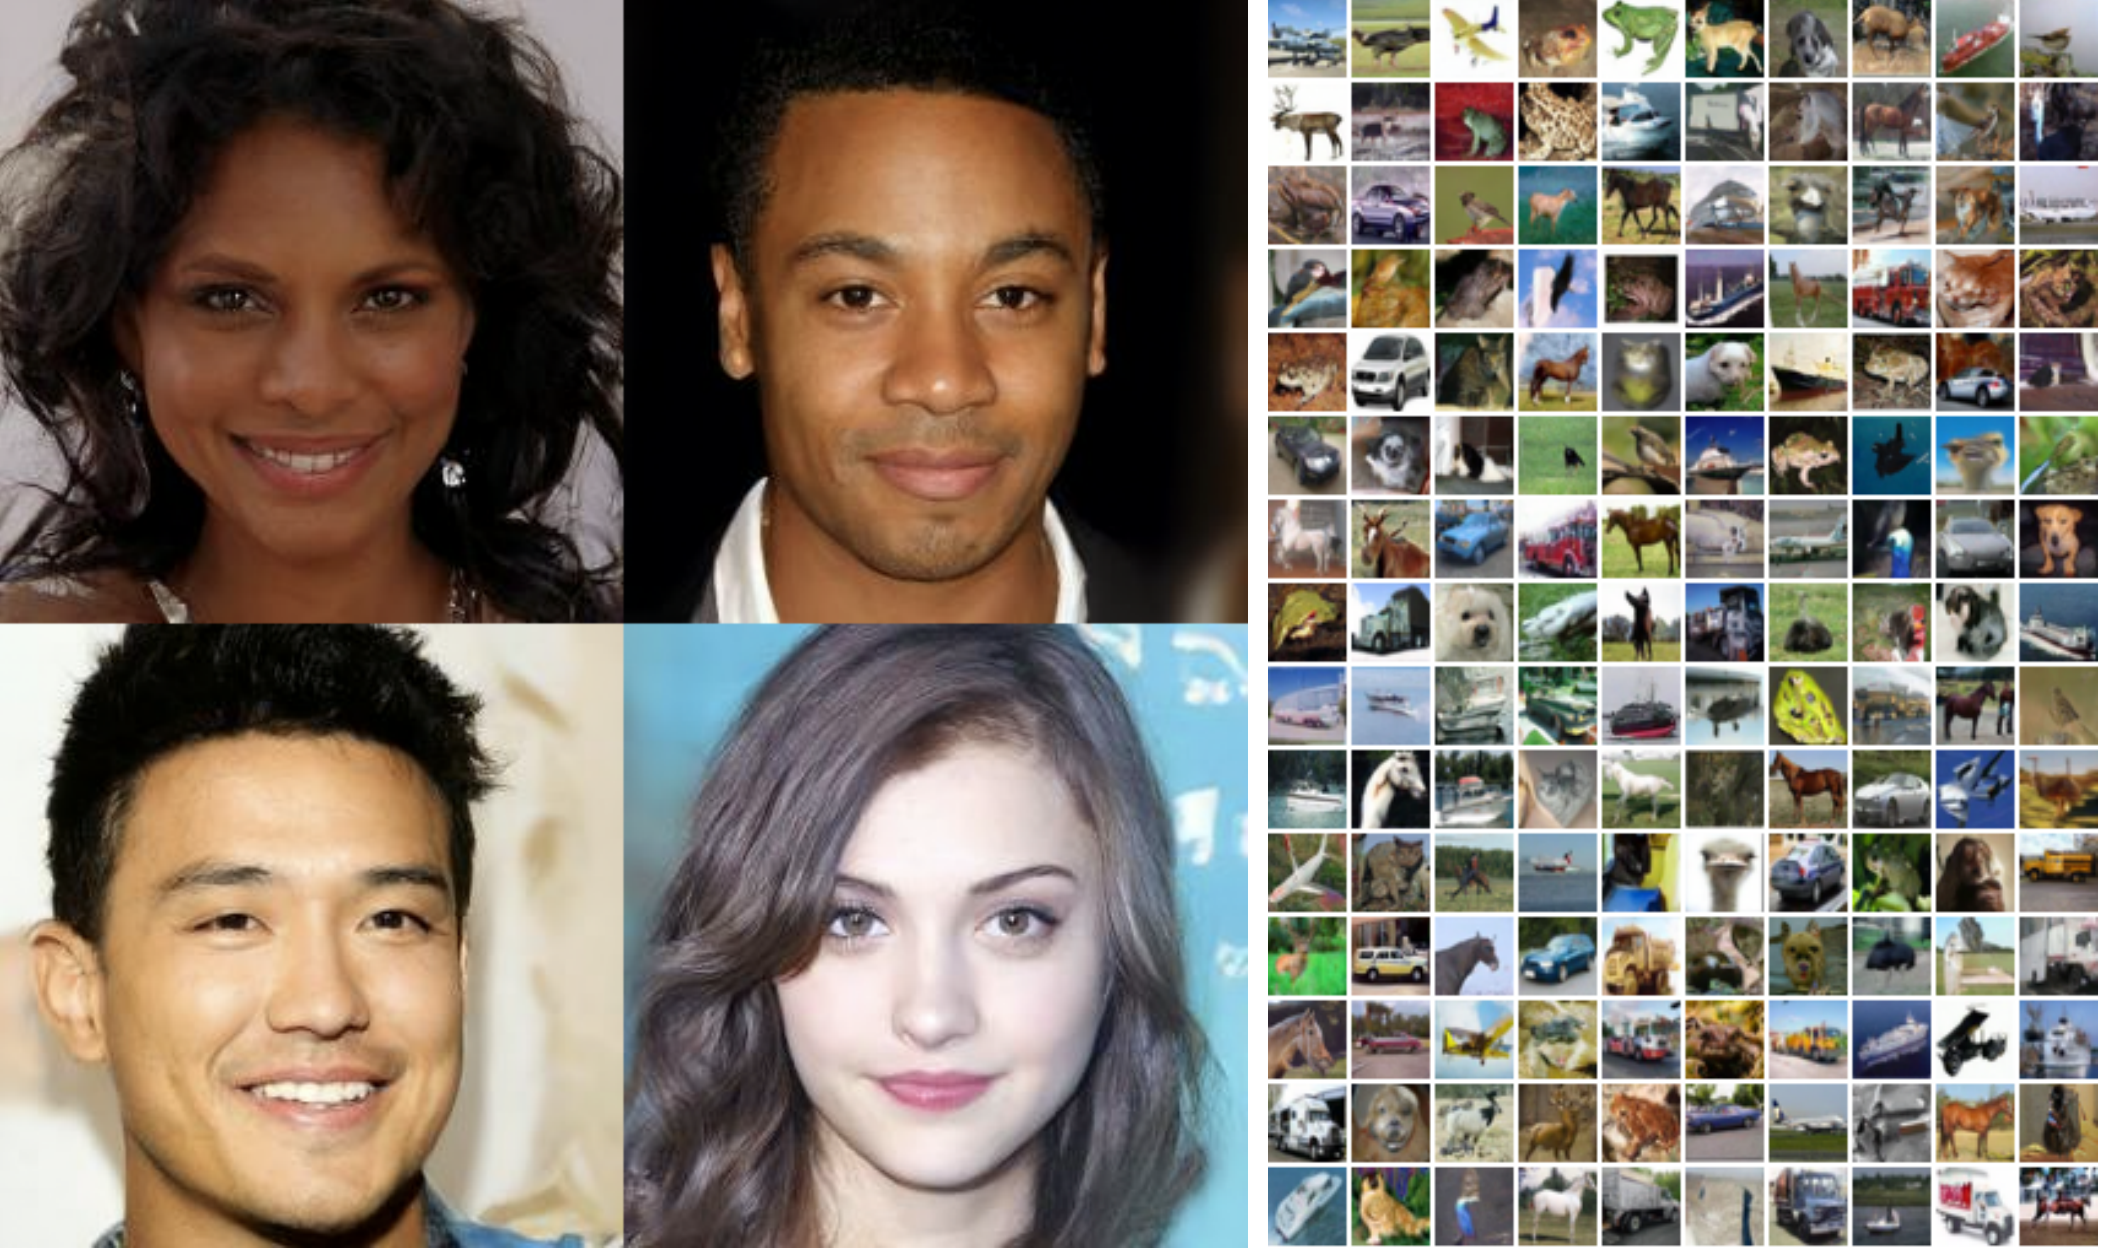
\includegraphics[width=\linewidth]{figs/ddpm_samples}
        \end{figure}
    \end{block}
\end{frame}
%=======
\begin{frame}{Summary}
    \begin{itemize}
        \item DDPM approximates the reverse process using normality assumptions.     
        \vfill
        \item DDPM can be interpreted as a VAE with a hierarchy of latent variables.
        \vfill
        \item The ELBO for DDPM may be formulated as a sum over many KL divergence terms.
        \vfill
        \item At each step, DDPM predicts the noise that was injected in the forward process. 
        \vfill
        \item DDPM is a VAE model that tries to invert the forward diffusion process via variational inference. 
        \vfill
        \item DDPMs are quite slow, since the model must be applied $T$ times for sampling.
    \end{itemize}
\end{frame}
%=======
\end{document}